%\documentclass[11pt,fleqn,twoside]{article}
\documentclass{llncs}

\usepackage[english]{babel}
\usepackage{alltt}
\usepackage{graphicx}
\usepackage{url}
\usepackage{subfigure}
\usepackage{listings}
\usepackage{color}
\usepackage{lscape}
\usepackage{xspace}
\usepackage{latexsym}
\usepackage{rotating} 
\usepackage{enumitem}

\usepackage{verbatim}
\usepackage{url}
\usepackage{multirow} 


\usepackage{colortbl}
\usepackage[table]{xcolor}

\makeatletter
\renewcommand{\thetable}{\thesection.\@arabic\c@table}
\@addtoreset{table}{section}
\makeatother


\definecolor{MyDarkBlue}{rgb}{0,0.08,0.45} 
\newcommand{\dv}[1] {\textcolor{blue}{[DV]\textit{#1}}}
\newcommand{\bo}[1] {\textcolor{MyDarkBlue}{[BO]\textit{#1}}}

\begin{document}

\title{Notes on Physical \& Logical Data Layouts}
	\author{
	Michael Hausenblas\inst{1} 
	}
	\institute{MapR Technologies EMEA, Ireland\\
	\email{mhausenblas@maprtech.com}
	}
\maketitle

\begin{abstract}
This article discusses principled options for physical and logical data layouts
and their implications on data processing at large scales. I should say in 
advance that these notes offer no new insights, that is, everything stated here 
has already been published elsewhere. In fact, it has been published in so many 
different places, such as blog posts, in the literature, mentioned at talks, 
spread over YouTube and Vimeo videos, uttered in hallway discussions and 
various whiteboards that its main contribution is to bring it all together in 
one place. The reader is expected to have a basic understanding in data 
management, databases and datastores as well as datashapes in general.
\end{abstract}

\section{Motivation}
\label{sec:mot}


\section{Manifestations of Data Layouts}
\label{sec:mani}

\begin{figure}[h!]
\centering
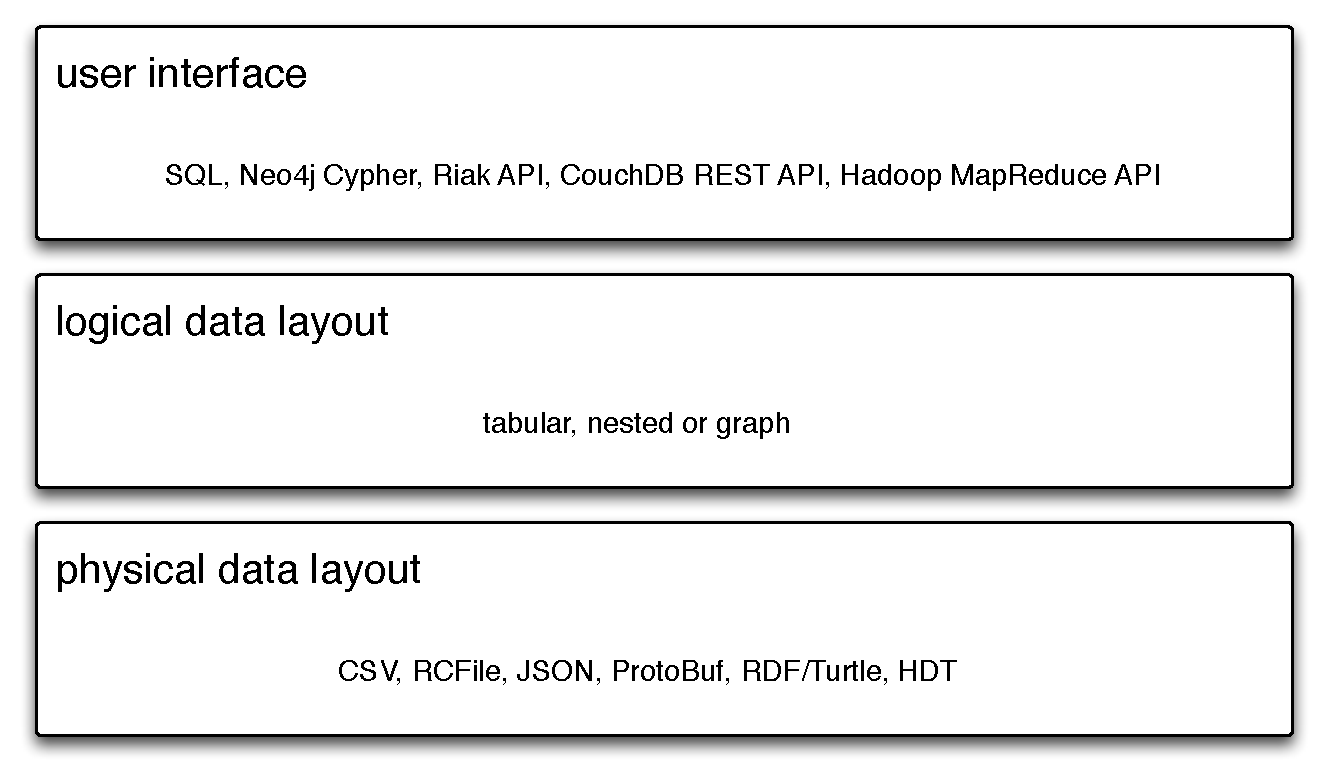
\includegraphics[width=0.5\textwidth]{data-layers}
\caption{The three layers of data representation and interaction.}
\label{fig:data-layers}
\end{figure}


\begin{figure}[h!]
\centering
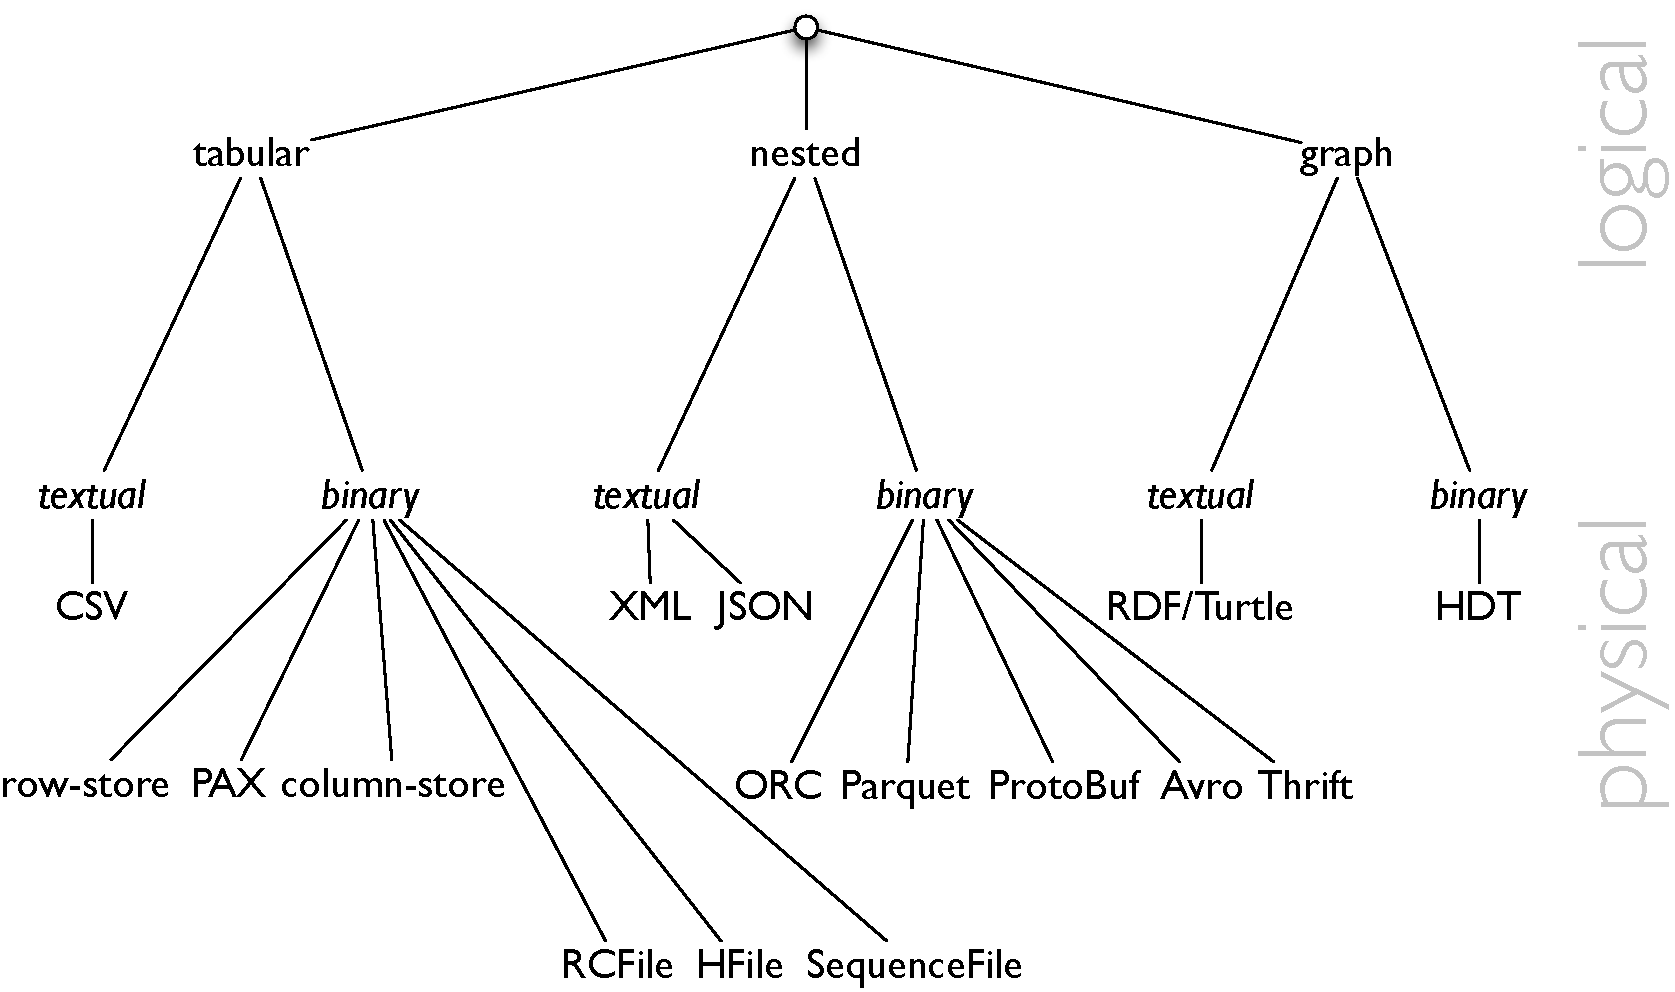
\includegraphics[width=0.9\textwidth]{taxonomy-dl}
\caption{A non-exhaustive, lightweight taxonomy for logical and physical data layouts and 
serialisation formats commonly used in the data processing community.}
\label{fig:taxonomy-dl}
\end{figure}

\section{Logical Layouts}
\label{sec:loglay}

\section{Physical Layouts}
\label{sec:phylay}

\section{Layering Physical and Logical Layouts}
\label{sec:laylay}


\section{Impact on Data Processing at Scale}
\label{sec:ldp}


\section{Conclusions and Challenges}
\label{sec:concl}


\bibliographystyle{alpha}
\bibliography{data-proc}


\end{document}

